
\section{Feral Mechanisms in Rails}
\label{sec:rails-cc}

As we discussed in Section~\ref{sec:deployment}, Rails services user
requests entirely independently, with the database acting as a point
of rendezvous for concurrent operations. Given Rails's design goals of
maintaining application logic at the user level, this appears---on its
face---a somewhat cavalier proposition with respect to application
integrity. In response, Rails has developed a range of concurrency
control strategies, two of which operate external to the database and
at the application level, which we term \textit{feral concurrency
  control} mechanisms.

In this section, we outline four major mechanisms for guarding against
integrity violations under concurrent execution in Rails. We
subsequently begin our study of 67 open source applications to
determine which of these mechanisms are used in practice. In the following
section, we will determine which are sufficient to maintain
correct data---and when they are not.

\subsection{Rails Concurrency Control Mechanisms}

Rails contains four main mechanisms for concurrency control.

\begin{myenumerate}
\item Rails provides support for \textbf{transactions}. By wrapping a
sequence of operations within a special \texttt{transaction} block,
Rails operations will execute transactionally, backed by an actual
database transaction. The database transaction either runs at the
database's configured default isolation level or, as of Rails 4.0.0, can
be configured on a per-transaction
basis~\cite{code-transaction-isolation}.

\item Rails provides support for both optimistic and pessimistic
  per-record \textbf{locking}. Applications invoke pessimistic locks
  on an Active Record object by calling its \texttt{lock} method,
  which invokes a \texttt{SELECT FOR UPDATE} statement in the
  database. Optimistic locking is invoked by declaring a special
  \texttt{lock\_version} field in an Active Record model. When a Rails
  process performs an update to an optimistically locked Model, Active
  Record atomically checks that an object's \texttt{lock\_version} has
  not changed since the process last read the object and, if it has
  not changed, transactionally increments \texttt{lock\_version} and updates the
  object in the database.

\item Rails provides support for application-level
  \textbf{validations}. Each Model has a set of zero or more
  validations, or boolean-valued functions that should be run before
  the object is actually saved to the database. A model instance many
  only be saved to the database if all of its declared validations
  return true. These validations ensure, for example, that particular
  fields within a record are not null or, alternatively, are unique
  within the database. Rails provides a number of built-in validators
  but also allows arbitrary user-defined validations (we discuss
  actual validations further in subsequent sections). Each validation
  declared for a given model is run sequentially within a
  database-backed transaction before actually updating the model state
  in the database.\footnote{The practice
    of wrapping validations in a transaction dates to the earliest public
    Rails commit (albeit, in 2004, transactions were only supported via a
    per-Ruby VM global lock~\cite{code-txn-lock}). However,
    as late as 2010, updates were only partially protected by
    transactions~\cite{code-txn-update}.}\\[-2mm]

  Rails validations are a prominent feature of the Active Record
  model. In contrast, neither transactions nor locks are actually
  discussed in the official ``Rails Guides,'' and, generally, are not
  promoted as a means of ensuring data integrity. Instead, the Rails
  documentation~\cite{rails-guide} prefers validations as they are
  ``are database agnostic, cannot be bypassed by end users, and are
  convenient to test and maintain.'' Moreover, the Rails documentation
  opines that ``[d]atabase constraints and/or stored procedures make
  the validation mechanisms database-dependent and can make testing
  and maintenance more difficult.'' As we will see in the next
  subsection, validations are widely used by many actual applications.

\item Rails provides support for application-level
  \textbf{associations}. Like validations, associations are a core
  concept of the Active Record model. As the name suggests, ``an
  association is a connection between two Active Record models,''
  effectively acting like a foreign key in an RDBMS. Associations can be declared on one or both sides of a
  one-to-one or one-to-many relationship, including transitive
  dependencies (via a \texttt{:through} annotation). Declaring an
  association (e.g., \texttt{:belongs\_to dept}) produces a special
  field for the associated record ID within the model (e.g.,
  \texttt{dept\_id}). Coupling an association with an appropriate
  validation (e.g., \texttt{:presence}) ensures that the association
  is indeed valid (and is, via the validation, backed by a database
  transaction). Rails does not currently provide native support for
  database-backed foreign key constraints.\footnote{However, Rails 4.2
    (in Beta as of November 2014) will add support for foreign key
    constraints via manual schema annotation.}
\end{myenumerate}

Overall, these four mechanisms provide a range of options for
developers. The first is squarely in the realm of traditional
concurrency control. The second is, in effect, a coarse-grained
user-level implementation of single-record transactions via
database-level ``compare-and-swap'' primitives (implemented via
\texttt{SELECT FOR UPDATE}). However, the latter two---validations and
associations---operate, in effect, at the application level. Although
some validations, such as uniqueness validations, have natural analogs
in an RDBMS, the semantics of these validations in Rails are entirely
contained within the Rails code. In effect, from the database's
perspective, these validations exist external to the system and are
\textit{feral} concurrency control mechanisms. As we will show
shortly, these feral mechanisms dominate in terms of developer
popularity.

\subsection{Adoption in Practice}

To understand exactly how users interact with these
concurrency control mechanisms and determine which deserved more
study, we examined their usage in a portfolio of publicly available
open source applications. We find that validations and associations
are overwhelmingly the most popular forms of concurrency control.

\minihead{Application corpus} We selected 67 open source applications
built using Ruby on Rails and Active Record, representing a variety of
application domains, including eCommerce, customer relationship
management, retail point of sale, conference management, content
management, build management, project management, personal task
tracking, community management and forums, commenting, calendaring,
file sharing, Git hosting, link aggregation, crowdfunding, social
networking, and blogging. We sought projects with substantial
code-bases (average: 26,380 lines of Ruby) multiple contributors
(average: 69.2), and relative popularity (measured according to GitHub
stars) on the site. Table~\ref{table:app-summary} (in the Appendix)
provides a detailed overview.


While several of these applications are projects undertaken by
hobbyists, many are either commercially supported (e.g., Canvas LMS,
Discourse, Spree, GitLab) and/or have a large open source community
(e.g., Radiant, Comfortable Mexican Sofa, Diaspora). Undoubtedly, a
larger-scale commercial, closed-source Rails projects such as Twitter,
GitHub, or Airbnb might exhibit different trends than those we observe
here. However, in the open source domain, we believe these
applications represent a diverse selection of Rails use cases, and a
good-faith effort to obtain a representative sample of open source
Rails applications as hosted on GitHub.

\minihead{Mechanism usage} We performed a simple analysis of the
applications to determine how each of the concurrency control
mechanisms were used (see Appendix~\ref{sec:appendix-methodology} for more
methodological details).

Overwhelmingly, applications did not use transactions or locks
(Figure~\ref{fig:usages} and Table~\ref{table:app-summary}). On
average, applications used 0.13 transactions, 0.01 locks, 1.82
validations, and 3.30 associations per model (with an average of 29.1
models per application). While 46 (68.7\%) of applications used
transactions, 66 (98.5\%) used validations or associations. Only six
applications (8.9\%) used locks. Use of pessimistic locks was more than
twice as common as the use of optimistic locks.

Overall, we find that validations and associations are, respectively,
14 and 25 times more common than transactions and orders of magnitude
more common than locking. These feral mechanisms are---in keeping with
the Rails philosophy---favored by these application developers. That
is, rather than adopting the use of traditional transactional
programming primitives, Rails application writers chose to instead declaratively specify
correctness criteria and have the ORM system check the criteria for
them instead. It is unclear and even unlikely that these declarative
criteria are a complete specification of program correctness:
undoubtedly, some of these programs contain errors. However, from the
perspective of database usability and idiomatic web programming
patterns, this reliance on application-level correctness criteria
hints at an alternative developer mentality than users of traditional
database concurrency control.  We devote much of the remainder of this
work to examining exactly what these feral mechanisms are attempting
preserve (and whether they are actually correct in doing so).

\minihead{Understanding specific applications} Over the course of our
investigation, we found varying use of mechanisms across
applications.

For example, the eCommerce application Spree uses only
six transactions, one for each of $1.)$ canceling an order, $2.)$
approving an order (atomically setting the user ID and timestamp),
$3.)$ transferring shipments between fulfillment locations (e.g.,
warehouses), $4.)$ transferring items between shipments, $5.)$
transfering stock between fulfillment locations, and $6.)$ updating an
order's specific inventory status.

In an eCommerce application like Spree, one might expect (as in the
canonical banking example from database textbooks) the inventory count
for each item to be a hotspot for concurrency issues. We found that
performing differential addition and subtraction to the available
stock of an item (\texttt{adjust\_count\_on\_hand(value)}) is indeed
protected via a pessimistic lock, but simply setting the available
stock (\texttt{set\_count\_on\_hand(value)}) is not. It is unclear why
one operation necessitates a lock but the other does not, given that
both are ostensibly sensitive to concurrent accesses. Meanwhile, the
stock level itself is wrapped in a validation ensuring non-negative
balances, if not Lost Updates.

At one point, Spree's inventory was protected by an optimistic lock;
it was removed due to optimistic lock failure during customer
checkouts. On relevant bug tracker issue, a committer notes that ``I
think we should get rid of the [optimistic lock] if there's no
documentation about why it's there...I think we can look at this issue
again in a month's time and see if there's been any problems since you
turned it off''~\cite{code-optimistic-issue}. The issue has, to our
knowledge, not been revisited, despite the potential dangers of
removing this point of synchronization.

Thus, the choice of (and even use of) concurrency control appears an
ad-hoc process. The remainder of the corpus contains a number of such
phenomena. The use of each style of concurrency control varies across
repositories, but our results demonstrate a clear trend towards feral
mechanisms within Rails rather than traditional use of
transactions. As a consequence of the breadth of our study (and paper
formatting limitations), we are not able to discuss every application
in detail (though the source code of each and, fortunately, the Git
history and issue trackers typically publicly available for
inspection).

\begin{figure}
  \newcommand{\skipht}{\\[-2em]}
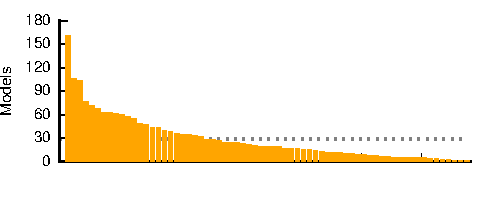
\includegraphics[width=\columnwidth]{figs/models-single-bar.pdf}\skipht
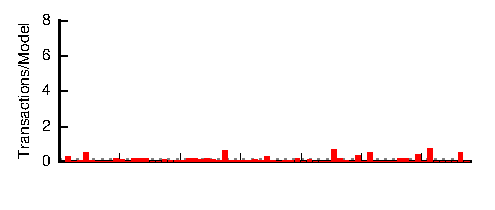
\includegraphics[width=\columnwidth]{figs/transactions-single-bar.pdf}\skipht
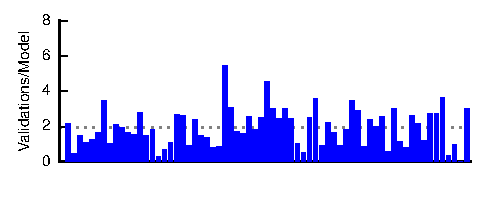
\includegraphics[width=\columnwidth]{figs/validations-single-bar.pdf}\skipht
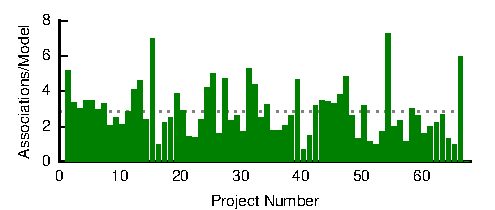
\includegraphics[width=\columnwidth]{figs/associations-single-bar.pdf}\skipht
\caption{Use of concurrency control mechanisms in Rails
  applications. We maintain the same ordering of applications for each
  plot (i.e., same x-axis values; identical to
  Table~\ref{table:app-summary}) and show the average for each plot
  using the dotted line.}
\label{fig:usages}
\end{figure}



\minihead{Additional metrics} To better understand how programmers
used each of these mechanisms, we report on two additional
analyses.

First, we analyzed the number of models, transactions, validations,
and associations over each project's lifetime. Using each
application's Git logs, we repeated the above analysis at a fixed set
of intervals through the application's history (by commits). At each
interval, we recorded the number of occurrences of each of these
constructs relative to the total number of occurrences in the project
in the latest repository we examined. Figure~\ref{fig:historical}
plots the median number of occurences across all projects. Notably,
these results demonstrate that, by the time 50\% of the commits have
been entered into the repository, over 75\% of the models,
transactions, validations, and associations have been written. This
suggests that the Model layer may be less volatile than the View and
Controller components of the applications. Moreover, the initial
proportion of validations and associations is higher than the initial
proportion of transactions; thus, the data model appears to stabilize
faster than the controller logic. It is unclear whether the bulk of
transaction usage is added in order to compensate for, say,
concurrency violations, or is instead due to growth in Controller code
and business logic.

\begin{figure}
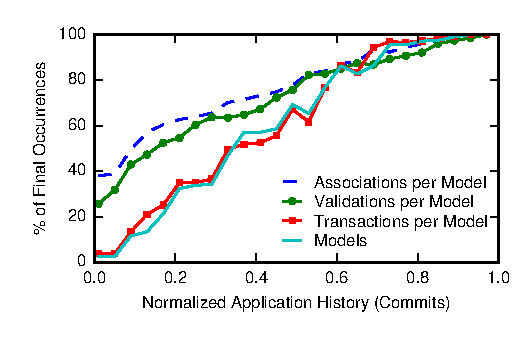
\includegraphics[width=\columnwidth]{figs/historical-median.pdf}\vspace{-2em}
\caption{Median use of Rails mechanisms over time.}
\label{fig:historical}
\end{figure}

Second, we analyze the distribution of authors to commits compared to
the distribution of authors to validations and associations
authored.\footnote{We chose to analyze commits authored rather than
  lines of code written because git tracks large-scale code
  refactoring commits as an often large set of deletions and
  insertions. Nevertheless, we observed a close correlation between
  lines of code and commits authored.} As Figure~\ref{fig:cdfs}
demonstrates, 95\% of all commits are authored by 42.4\% of
authors. However, 95\% of invariants (validations plus associations)
are authored by only 20.3\% of authors. This is reminiscent of
traditional database schema authorship, where a smaller number of
authors (e.g., DBAs) modify the schema than contribute to the actual
application code.

\begin{figure}
  \newcommand{\skipht}{\\[-2em]}
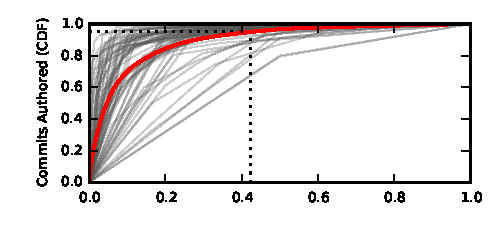
\includegraphics[width=\columnwidth]{figs/commit-authorship-cdf.pdf}\vspace{-2em}
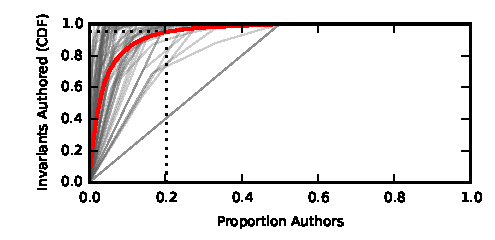
\includegraphics[width=\columnwidth]{figs/invariant-authorship-cdf.pdf}\vspace{-1em}
\caption{CDFs of authorship of invariants (validations plus
  associations) and commits. Bolded line
  shows the average CDF across projects, while faint lines show CDFs
  for individual projects. The dotted line shows the 95th percentile
  CDF value. }
\label{fig:cdfs}
\end{figure}

\subsection{Discussion}

Returning to the Rails design philosophy, the applications we have
encountered do indeed express their logic at the application
layer. There is little actual communication of correctness criteria to
the database layer. Part of this is due to limitations within
Rails. As we have mentioned, there is no way to actually declare a
foreign key constraint in Rails without importing additional
third-party modules. Insofar as Rails is an ``opinionated'' framework
encouraging an idiomatic programming style, if our application corpus
is any indication, DHH and his co-authors advocating application-level
data management appear to have succeeded en masse.

Having observed the relative popularity of these mechanisms, we turn
our attention to the question of their correctness. Specifically, do
these application-level criteria actually enforce the constraints that
they claim to enforce? We restrict ourself to studying declared
validations and associations for three reasons. First, as we have
seen, these constructs are more widely used in the codebases we have
studied. Second, these constructs represent a deviation from standard
concurrency control techniques and are therefore perhaps more likely
to contain errors. Third, while analyzing latent constraints (i.e.,
those that might be determined via more sophisticated techniques such
as pre- and post-condition invariant
mining~\cite{writes-forest,redblue-new} and/or by interviewing each
developer on each project) would be instructive, this is difficult to
scale. We view these forms of analysis as worthwhile avenues for
future research.
